\documentclass[11pt]{article}
\usepackage[margin=3cm]{geometry}
\usepackage[utf8]{inputenc}
\usepackage[english]{babel}
\usepackage{amsmath}
\usepackage{amssymb}
\usepackage{amsfonts}
\usepackage{xargs}
\usepackage[
    pdftex, 
    dvipsnames
]{xcolor}
\usepackage[
    colorlinks=true,
    linkcolor=black,
    urlcolor=Thistle,
    citecolor=DarkOrchid
]{hyperref}
\usepackage{fancyhdr}
\usepackage{datetime}
\usepackage{ccicons}
\usepackage{tikz}
\usepackage{cancel}
\usepackage{mdframed}
%\usepackage[outputdir=.texpadtmp]{minted}

% ==== License =====
\usepackage[
    type={CC}, 
    modifier={by-nc-sa}, 
    version={4.0},
]{doclicense}

% ==== todo notes ====
\usepackage[
    colorinlistoftodos,
    prependcaption,
    textsize=tiny
]{todonotes}
\newcommandx{\note}[2][1=]{\todo[linecolor=Thistle,backgroundcolor=Thistle!25,bordercolor=Thistle,#1]{#2}}
\newcommandx{\unsure}[2][1=]{\todo[linecolor=red,backgroundcolor=red!25,bordercolor=red,#1]{#2}}
\newcommandx{\change}[2][1=]{\todo[linecolor=blue,backgroundcolor=blue!25,bordercolor=blue,#1]{#2}}
\newcommandx{\info}[2][1=]{\todo[linecolor=OliveGreen,backgroundcolor=OliveGreen!25,bordercolor=OliveGreen,#1]{#2}}
\newcommandx{\improvement}[2][1=]{\todo[linecolor=Plum,backgroundcolor=Plum!25,bordercolor=Plum,#1]{#2}}

% General
\newcommand{\mc}[1]{\mathcal{#1}}
\newcommand{\argmax}{\arg\max}
\newcommand{\kl}{\mathrm{KL}}

\newenvironment{rcases}
  {\left.\begin{aligned}}
  {\end{aligned}\right\rbrace}

% Math Bold Font, Vector Notations
\newcommand{\ba}{\mathbf{a}}
\newcommand{\bb}{\mathbf{b}}
\newcommand{\bc}{\mathbf{c}}
\newcommand{\bd}{\mathbf{d}}
\newcommand{\be}{\mathbf{e}}
\renewcommand{\bf}{\mathbf{f}}
\newcommand{\bg}{\mathbf{g}}
\newcommand{\bh}{\mathbf{h}}
\newcommand{\bi}{\mathbf{i}}
\newcommand{\bj}{\mathbf{j}}
\newcommand{\bk}{\mathbf{k}}
\newcommand{\bl}{\mathbf{l}}
\newcommand{\bm}{\mathbf{m}}
\newcommand{\bn}{\mathbf{n}}
\newcommand{\bo}{\mathbf{o}}
\newcommand{\bp}{\mathbf{p}}
\newcommand{\bq}{\mathbf{q}}
\newcommand{\br}{\mathbf{r}}
\newcommand{\bs}{\mathbf{s}}
\newcommand{\bt}{\mathbf{t}}
\newcommand{\bu}{\mathbf{u}}
\newcommand{\bv}{\mathbf{v}}
\newcommand{\bw}{\mathbf{w}}
\newcommand{\bx}{\mathbf{x}}
\newcommand{\by}{\mathbf{y}}
\newcommand{\bz}{\mathbf{z}}
\newcommand{\bzero}{\mathbf{0}}

% Proofs, Structures
\newcommand{\proof}{\tit{\underline{Proof:}}} % This equivalent to the \begin{proof}\end{proof} block
\newcommand{\proofforward}{\tit{\underline{Proof($\implies$):}}}
\newcommand{\proofback}{\tit{\underline{Proof($\impliedby$):}}}
\newcommand{\proofsuperset}{\tit{\underline{Proof($\supseteq$):}}}
\newcommand{\proofsubset}{\tit{\underline{Proof($\subseteq$):}}}
\newcommand{\contradiction}{$\longrightarrow\!\longleftarrow$}
\newcommand{\qed}{\hfill $\blacksquare$}

% Number Spaces, Vector Space
\newcommand{\R}{\mathbb{R}}
\newcommand{\real}{\mathbb{R}}
\newcommand{\complex}{\mathbb{C}}
\newcommand{\field}{\mathbb{F}}

% customized commands
\newcommand{\settag}[1]{\renewcommand{\theenumi}{#1}}
\newcommand{\tbf}[1]{\textbf{#1}}
\newcommand{\tit}[1]{\textit{#1}}
\newcommand{\overbar}[1]{\mkern 1.5mu\overline{\mkern-1.5mu#1\mkern-1.5mu}\mkern 1.5mu}
\newcommand{\double}[1]{\mathbb{#1}} % Set to behave like that on word
\newcommand{\trans}[3]{$#1:#2\rightarrow{}#3$}
\newcommand{\map}[3]{\text{$\left[#1\right]_{#2}^{#3}$}}
\newcommand{\dime}[1]{\text{dim}(#1)}
\newcommand{\mat}[2]{M_{#1 \times #2}(\R)}
\newcommand{\aug}{\fboxsep=-\fboxrule\!\!\!\fbox{\strut}\!\!\!}
\newcommand{\basecase}{\textsc{\underline{Basis Case:}} }
\newcommand{\inductive}{\textsc{\underline{Inductive Step:}} }
\newcommand{\norm}[1]{\left\lVert#1\right\rVert}
\newcommand{\independent}{\perp}

\usepackage{chngcntr}
\counterwithin{figure}{section}
\counterwithin{table}{section}
\counterwithin{equation}{section}

\author{\ccLogo \,\,by Xia, Tingfeng}
\title{\textsc{Statistical Methods for Machine Learning II}}
\date{2020 winter term}

\begin{document}
\maketitle
\doclicenseThis

\section*{Preface} 
This document is consist of notes from lectures and the online course notes that I, personally, find interesting/important. You can find the online course notes on the course website here: \url{https://probmlcourse.github.io/sta414/}

\tableofcontents

\newpage

\section{Lecture 2 - Introduction to Probabilistic Models}
\subsection{Overview}
We have a random vector in the form $X = (X_1,\dots,X_m)$ which can be \textit{\textbf{either observed or unobserved}}. To approach this in a generative way, we make the so called generative assumption. which is that $X\sim P_{true}(X)$, i.e. there is some true distribution that is behind the scene and our data is from such distribution. 

\paragraph{Goal} Model a parametric joint distribution $P_\theta (X)$ by learning the parameters. The learning here means we want to find a/the ``close''/``best'' estimation to our parameter $\theta$. In this course we will investigate the following three problems,
\begin{itemize}
    \item How to specify the joint, $P_\theta(X)$?
    \item What does ``best''/``close'' mean? In some sense we want to find $P_\theta \approx P_{true}$, however $P_{true}$ might also be unknown.
    \item How to find the best $\theta$? In this course we will generally rely on gradient methods, so $\nabla_\theta$...
\end{itemize}

\subsection{Probabilistic Perspective on ML}
With this perspective, we can think about common machine learning tasks differently, where random variables represent:
\begin{itemize}
    \item $X$: (high dimensional) input data
    \item $C$: discrete label
    \item $Y$: continuous target
\end{itemize}
If we assume our knowledge of the joint of the above three, i.e. we know $P(X,C,Y)$, then we can write our familiar tasks in the following way
\begin{itemize}
    \item \textit{\textbf{Regression}}:
        \begin{equation}
            p(Y|X) = \frac{p(X,Y)}{P(X)} = \frac{p(X,Y)}{\int p(X,Y)dY}
        \end{equation}
    \item \textit{\textbf{Classification/Clustering}}:
        \begin{equation}
            p(C|X) = \frac{p(X,C)}{\sum_{C'}p(X,C')}
        \end{equation}
\end{itemize}

\subsubsection{(Example) Classification} Suppose we have data of the form $\mathcal{D} = \{(x,c)_i\}_i$. We assume that they came from a certain true distribution, i.e. $\{(x,c)_i\}_i \sim p(X,C)$. Then, the ultimate goal of the ML problem is converted into finding $p(C|X)$. Using Bayes Rule of total probability, we can expand the distribution of interest into
\begin{equation}
    p(C | X)= \frac{p(X,C)}{P(X)} =\frac{p(X, C)}{\sum_{C'} p(X, C')}
\end{equation}

\paragraph{Output Heuristics} After we acquire $p(C|X)$ as above, we are one step away from our goal of output the actual prediction $c^*$. There are three ways that we can do this, namely
\begin{itemize}
    \item \textit{\textbf{MLE Estimate}} is the most intuitive one, we simply choose
        \begin{equation}
            c^* = \argmax_c p(C = c|X)
        \end{equation}
    \item \textit{\textbf{Sample Learnt Dist}} is another approach which produces non-deterministic results, i.e. we sample $c^* \sim p(C|X)$.
    \item \textit{\textbf{Combined}} is usually a safe way of doing this. We output
        \begin{equation}
            (c^*, p(C=c^*|X)) \iff (\text{result}, \text{how sure?})
        \end{equation}
    As an example, we have a ML algorithm drives a car. In this case, we might want to make decision only when the machine learning model has a certain level of confidence. 
\end{itemize}

\subsection{Observed vs Unobserved Random Variables}
\subsubsection{Supervised Dataset}
\begin{equation}
    \left\{x_{i}, c_{i}\right\}_{i=1}^{N} \sim p(X, C)
\end{equation}
In such case, the class labels are observed and finding the conditional distribution $p(C|X)$ satisfies the supervised classification problem. 

\subsubsection{Unsupervised Dataset}
\begin{equation}
    \left\{x_{i}\right\}_{i=1}^{N} \sim p(X, C)
\end{equation}
Still under the generative assumption, where we assume that there is some underlying distribution for our dataset. Further, we assume that the distribution of data is related to the class labels for the data points even though the class labels are never observed. \textbf{A common way to refer to an unobserved discrete class label is ``cluster''}. However, in this case, our final goal of classification is still $p(C|X)$\footnote{Might be helpful to think of Gaussian Mixture Models}. 

\subsubsection{Latent Variables} 
\begin{quote}
    Further, like clusters, introducing assumptions about unobserved variables is a powerful modelling tool. We will make use of this by modelling variables which are never observed in the dataset, called latent or hidden variables. By introducing and modelling latent variables, we will be able to naturally describe and capture abstract features of our input data.
\end{quote}

\subsection{Operations on Probabilistic Models}
\begin{itemize}
    \item \textit{\textbf{Generate Data}}: Sample from the model.
    \item \textit{\textbf{Estimate Likelihood}}: When all variables are either observed or marginalized, we produce the result which is a single real number that describes the `probability' of the all variables taking on those specific values.
    \item \textit{\textbf{Inference}}: Compute the expected value of some variables given others which are either observed or marginalized. 
    \item \textit{\textbf{Learning}}: Set the parameters of the joint distribution given some observed data to maximize the probability of the observed data. 
\end{itemize}

\subsection{Desiderata of Probabilistic Models}
We have two desires for the joint distribution to learn, namely
\begin{itemize}
    \item The marginal and conditional distribution can be computed efficiently
    \item The representation of the joint distribution should be compact. This is especially important when we are dealing with joint distributions over many variables.
\end{itemize}
In general, total joint distribution are too large to specify and would require an insane amount of data to fit even we wanted to. Thus, we need modelling assumptions. 

\subsubsection{Fully Dependent Factorization (Chain Rule)}
Suppose we have sample space defined such that $|T| = 2$, $|W| = 3$, and $|M| = 4$. Then the total joint distribution could be expanding using the chain rule as (\textit{note: not unique})
\begin{equation}
    P_\theta(T,W,M) = P(T)P(W|T)P(M|T,W)
\end{equation} 
which requires\footnote{Here the bars mean ``cardinality'' rather than vector norm} $|\theta| = (2 - 1) + (3 - 1) \times 2 + (4 - 1)\times 2 \times 3 = 23$ parameters in total to specify. 

\subsubsection{Assumptions (Independence)}
Introducing assumptions results in
\begin{itemize}
    \item a less expressive model
    \item $|\theta|$ (usually, much) smaller
\end{itemize}
which can be bad sometimes (since the model is less expressive) and is a trade-off that we as modellers have to deal with. 

\paragraph{(Example) Fully Independent}
We assume that $T\independent W \independent M$, then by definition we know, for example, $P(W|T)= P(W)$. Then
\begin{align}
    P_\theta(T,W,M) &= P(T)P(W|T)P(M|T,W) \\
    &= P(T)P(W)P(M)
\end{align}
which requires only $|\theta| = (2-1) + (3-1) + (4-1) = 6$ to fit.

\subsection{Likelihood Function}
For some observed data $X$, the likelihood describes the likeliness of the data under then distribution with parameter $\theta$. 
\begin{equation}
    L(\theta) = p(X|\theta)
\end{equation}

In general, we prefer to deal with the log likelihood function, which is defined as
\begin{equation}
    \ell(\theta;X) = \log L(\theta) = \log p(X|\theta)
\end{equation}

\subsection{Maximum Likelihood Estimation}
The idea is to find
\begin{equation}
    \hat{\theta}_{MLE} := \argmax_\theta \ell(\theta; \mathcal{D})
\end{equation}
In the case of i.i.d, we can re-write as
\begin{align}
    \hat{\theta}_{MLE} &= \argmax_\theta \ell(\theta; \mathcal{D})\\
    &= \argmax_\theta \log \prod_{m} p\left(x^{(m)} | \theta\right) \\
    &= \argmax_\theta\sum_{m} \log p\left(x^{(m)} | \theta\right)
\end{align}

\subsection{Sufficient Statistics}
\paragraph{(Definition) Statistic}
A statistic is a possibly vector valued \textit{deterministic} function of a set of random variables.

\paragraph{(Definition) Sufficient Statistic} 
is a statistic that conveys exactly the same information about the data generating process that created the data as the entire data itself.\footnote{Could also be interpreted as ``summarize the data with respect to the likelihood''} In formal language, Sufficient Statistic ($T(X)$) for $X$ could be defined as
\begin{equation}
    T(X^{(1)}) = T(X^{(2)})~ \implies~ L(\theta; X^{(1)}) = L(\theta; X^{(2)}), ~~\forall \theta
\end{equation}
alternatively, we can define it as
\begin{equation}
    P(\theta | T(X)) = P(\theta | X); ~~~\text{\color{Gray} i.e. data doesn't give further info}
\end{equation}
\subsubsection{Fisher-Neyman Factorization Theorem}
If the probability function is $f_\theta(x)$, then $T$ is a sufficient statistic for $\theta$ if and only if non-negative functions $g$ and $h$ can be found such that
\begin{equation}
    P(\theta | T(X))=h(x, T(x)) g(T(x), \theta)
\end{equation}

\subsection{Exponential Family}
Factorizes as
\begin{align}
    p(x | \eta) 
    &=h(x) \exp \left\{\eta' T(x)-g(\eta)\right\} \\
    &=h(x) g(\eta) \exp \left\{\eta' T(x)\right\}
\end{align}
\subsubsection{(Example) 1-D Gaussian}
\begin{align}
    p(x|\theta) = \mathcal{N}(x|\mu, \sigma)
    &= \frac{1}{\sqrt{2\pi \sigma^2}}\exp \left(- \frac{1}{2\sigma^2} (x - \mu)^2 \right) \\
    &= \frac{1}{\sqrt{2\pi \sigma^2}}\exp \left(- \frac{1}{2\sigma^2} (x^2 - 2x\mu + \mu^2) \right) \\
    &= 
        \underbrace{\frac{1}{\sqrt{2\pi}\sigma}}_{h(x)} 
        \underbrace{\exp\left( \frac{-\mu^2}{2\sigma^2} \right)}_{g(\eta)}
    \exp\left(
    \underbrace{
        \begin{bmatrix}
            \frac{\mu}{\sigma^2} 
            & \frac{-1}{2\sigma^2}
        \end{bmatrix}}_{\eta}
    \underbrace{
        \begin{bmatrix}
            x \\
            x^2
        \end{bmatrix}}_{T(X)}
    \right)
\end{align}



\section{Lecture 3 - Directed Graphical Models}
\subsection{Decision Theory (Utility Theory)}
Let $a$ denote action, and $a^*$ be the optimal one. Also use $s$ to denote state and $V(\cdot)$\note{Often, it is very hard to find a/the good/best value function that quantifies everything using a numerical value. } be the value function. We have, in general
\begin{equation}
    a^* = \arg\min_a/\argmax_a \underbrace{{\mathbb{E}}_{p(s\vert a, knowledge)}\left[V(s)\right]}_{u(a)~ \overset{\Delta}{=} ~\text{utility of action $a$}}
\end{equation}

\subsection{Graphical Model Notation}
\subsubsection{Chain Rule Expansion} Given any joint probability of $N$ random variables, we can expand it as follows
\begin{equation}
    p\left(x_{1, \ldots, N}\right)=p\left(x_{1}\right) p\left(x_{2} | x_{1}\right) p\left(x_{3} | x_{2}, x_{1}\right) \ldots p\left(x_{n} | x_{n-1: 1}\right)
\end{equation}
Formally speaking, in the case of two random variables would simply
\begin{equation}
    p(x, y)=p(x | y) p(y)
\end{equation}
and the general case for $N$ random variables could be written as
\footnote{Note: when $k = 1$, $p\left(x_{k} | \cap_{j=1}^{k-1} x_{j}\right) = p(x_1)$}
\begin{equation}
    p\left(\bigcap_{i=1}^{N} x_{i}\right)
    = \prod_{j=1}^{N} p\left(x_{j} \left\vert\,\, \bigcap_{k=1}^{j-1} x_{k}\right)\right.
\end{equation}

\subsubsection{Graph Representation} 
\paragraph{(Example) Grouping Variables} Consider the model
\begin{equation}
    p\left(x_{i}, x_{\pi_{i}}\right)=p\left(x_{\pi_{i}}\right) p\left(x_{i} | x_{\pi_{i}}\right)
\end{equation}
which we can use the following graph to represent:
\begin{center}
    \begin{tikzpicture}[scale=0.2]
        \tikzstyle{every node}+=[inner sep=0pt]
        \draw [black] (25.7,-27.6) circle (3);
        \draw (25.7,-27.6) node {$x_{\pi_1}$};
        \draw [black] (41.1,-27.6) circle (3);
        \draw (41.1,-27.6) node {$x_1$};
        \draw [black] (28.7,-27.6) -- (38.1,-27.6);
        \fill [black] (38.1,-27.6) -- (37.3,-27.1) -- (37.3,-28.1);
    \end{tikzpicture}
\end{center}
where
\begin{itemize}
    \item \textit{\textbf{nodes}} represent random variables
    \item \textit{\textbf{arrows}} mean ``conditioned on'', e.g. ``$x_i$ is conditioned on $x_{\pi_i}$''
\end{itemize}
Notice that we can always group the variables together into one bigger variable, so in this example, $x_{\pi_i}$ might represent a group of variables in stead of just one. 


\paragraph{(Example) Fully Dependent 6 Nodes}
The total expansion of $p(x_{1:6})$ could be represented as
\begin{center}
    \begin{tikzpicture}[scale=0.2]
        \tikzstyle{every node}+=[inner sep=0pt]
        \draw [black] (19.3,-19.9) circle (3);
        \draw (19.3,-19.9) node {$x_1$};
        \draw [black] (36.4,-15.5) circle (3);
        \draw (36.4,-15.5) node {$x_2$};
        \draw [black] (53.6,-19.9) circle (3);
        \draw (53.6,-19.9) node {$x_3$};
        \draw [black] (53.6,-31.7) circle (3);
        \draw (53.6,-31.7) node {$x_4$};
        \draw [black] (19.3,-31.7) circle (3);
        \draw (19.3,-31.7) node {$x_6$};
        \draw [black] (36.4,-36.4) circle (3);
        \draw (36.4,-36.4) node {$x_5$};
        \draw [black] (22.21,-19.15) -- (33.49,-16.25);
        \fill [black] (33.49,-16.25) -- (32.6,-15.96) -- (32.84,-16.93);
        \draw [black] (22.3,-19.9) -- (50.6,-19.9);
        \fill [black] (50.6,-19.9) -- (49.8,-19.4) -- (49.8,-20.4);
        \draw [black] (22.14,-20.88) -- (50.76,-30.72);
        \fill [black] (50.76,-30.72) -- (50.17,-29.99) -- (49.84,-30.94);
        \draw [black] (21.46,-21.98) -- (34.24,-34.32);
        \fill [black] (34.24,-34.32) -- (34.01,-33.4) -- (33.32,-34.12);
        \draw [black] (19.3,-22.9) -- (19.3,-28.7);
        \fill [black] (19.3,-28.7) -- (19.8,-27.9) -- (18.8,-27.9);
        \draw [black] (39.31,-16.24) -- (50.69,-19.16);
        \fill [black] (50.69,-19.16) -- (50.04,-18.47) -- (49.79,-19.44);
        \draw [black] (38.58,-17.56) -- (51.42,-29.64);
        \fill [black] (51.42,-29.64) -- (51.18,-28.73) -- (50.49,-29.46);
        \draw [black] (36.4,-18.5) -- (36.4,-33.4);
        \fill [black] (36.4,-33.4) -- (36.9,-32.6) -- (35.9,-32.6);
        \draw [black] (34.22,-17.56) -- (21.48,-29.64);
        \fill [black] (21.48,-29.64) -- (22.4,-29.45) -- (21.71,-28.72);
        \draw [black] (53.6,-22.9) -- (53.6,-28.7);
        \fill [black] (53.6,-28.7) -- (54.1,-27.9) -- (53.1,-27.9);
        \draw [black] (51.44,-21.98) -- (38.56,-34.32);
        \fill [black] (38.56,-34.32) -- (39.49,-34.13) -- (38.8,-33.41);
        \draw [black] (50.76,-20.88) -- (22.14,-30.72);
        \fill [black] (22.14,-30.72) -- (23.06,-30.94) -- (22.73,-29.99);
        \draw [black] (50.71,-32.49) -- (39.29,-35.61);
        \fill [black] (39.29,-35.61) -- (40.2,-35.88) -- (39.93,-34.92);
        \draw [black] (50.6,-31.7) -- (22.3,-31.7);
        \fill [black] (22.3,-31.7) -- (23.1,-32.2) -- (23.1,-31.2);
        \draw [black] (33.51,-35.6) -- (22.19,-32.5);
        \fill [black] (22.19,-32.5) -- (22.83,-33.19) -- (23.1,-32.22);
    \end{tikzpicture}
\end{center}
This is the resultant graphical model if we make \textit{\textbf{absolutely no assumption}} on the independence. Notice that such model grows exponentially in complexity with respect to the number of parameters considered. We say such model ``scales poorly''.

\subsubsection{Conditional Independence} 
\paragraph{(Definition) Conditional Independence} Let $X$ be the set of nodes in our graph (the random variables of our model), then two sets of variables $X_A, X_B$ are said to be conditionally independent given a third set of variables $X_C$ if and only if either
\begin{equation}
    p\left(X_{A}, X_{B} | X_{C}\right)=p\left(X_{A} | X_{C}\right) p\left(X_{B} | X_{C}\right)
\end{equation}
or (\textit{\textbf{\#! Important!}})
\begin{align}
    &p\left(X_{A} | X_{B}, X_{C}\right)=p\left(X_{A} | X_{C}\right) \\
    \iff &p\left(X_{B} | X_{A}, X_{C}\right)=p\left(X_{B} | X_{C}\right)
\end{align}
and we denote the relation as $\left(X_{A} \independent X_{B} | X_{C}\right)$

\subsubsection{Plates}
In Bayesian methods, we treat parameters as random variables and hence we would like to include them in out graphical model. However, adding a node for each observation is quite cumbersome and thus we introduce plates, which denote replication of random variables. 

\paragraph{Nested Plates}
Plates could be nested, in which case their arrows get duplicated also, \textit{\textbf{according to the rule:}} draw an arrow from every copy of the source node to every copy of the destination node.

\paragraph{Crossing Plates}
Plates can also cross (intersect), in which case the nodes at the intersection have multiple indices and get duplicated a number of times equal to the product of the duplication numbers on all the plates containing them.


\subsection{Directed Acyclic Graphical Models (DAGM)}
A directed acyclic graphical model over $N$ random variables look like
\begin{equation}
    p\left(x_{1:N}\right)=\prod_{i}^{N} p\left(x_{i} | x_{\pi_{i}}\right)
\end{equation}
where $x_i$ is a random variable and $x_{\pi_i}$ denotes the parents of the node (which could be an empty set). This notion is more general than the fully dependence model that looked at above. Notice that here each node is only dependent on its parents rather than all other nodes. Thus, the complexity of such model reduces to exponential in fan-in of each node, instead of the total $N$. 

\subsubsection{Independence Assumption on DAGMs}
% TODO: Topological Sort?
Then, we have the independence relationship of\footnote{Requires topological ordering, to be added later. }
$
    x_i \independent x_{Ancestor({\pi_i})} \vert x_{\pi_i}
$
which expands into
\begin{equation}
    p\left(x_{1, \ldots, 6}\right)=p\left(x_{1}\right) p\left(x_{2} | x_{1}\right) p\left(x_{3} | x_{1}\right) p\left(x_{4} | x_{2}\right) p\left(x_{5} | x_{3}\right) p\left(x_{6} | x_{2}, x_{5}\right)
\end{equation}
with the following respective graph
\begin{center}
    \begin{tikzpicture}[scale=0.2]
        \tikzstyle{every node}+=[inner sep=0pt]
        \draw [black] (19.3,-19.9) circle (3);
        \draw (19.3,-19.9) node {$x_1$};
        \draw [black] (36.4,-15.5) circle (3);
        \draw (36.4,-15.5) node {$x_2$};
        \draw [black] (53.6,-19.9) circle (3);
        \draw (53.6,-19.9) node {$x_3$};
        \draw [black] (53.6,-31.7) circle (3);
        \draw (53.6,-31.7) node {$x_4$};
        \draw [black] (19.3,-31.7) circle (3);
        \draw (19.3,-31.7) node {$x_6$};
        \draw [black] (36.4,-36.4) circle (3);
        \draw (36.4,-36.4) node {$x_5$};
        \draw [black] (22.21,-19.15) -- (33.49,-16.25);
        \fill [black] (33.49,-16.25) -- (32.6,-15.96) -- (32.84,-16.93);
        \draw [black] (34.22,-17.56) -- (21.48,-29.64);
        \fill [black] (21.48,-29.64) -- (22.4,-29.45) -- (21.71,-28.72);
        \draw [black] (38.58,-17.56) -- (51.42,-29.64);
        \fill [black] (51.42,-29.64) -- (51.18,-28.73) -- (50.49,-29.46);
        \draw [black] (22.3,-19.9) -- (50.6,-19.9);
        \fill [black] (50.6,-19.9) -- (49.8,-19.4) -- (49.8,-20.4);
        \draw [black] (51.44,-21.98) -- (38.56,-34.32);
        \fill [black] (38.56,-34.32) -- (39.49,-34.13) -- (38.8,-33.41);
        \draw [black] (33.51,-35.6) -- (22.19,-32.5);
        \fill [black] (22.19,-32.5) -- (22.83,-33.19) -- (23.1,-32.22);
    \end{tikzpicture}
\end{center}
As we can see, the introduction of the assumption greatly reduced the complexity of the model. 
\subsubsection{(Example) Markov Chain}
The following example has independence relationships that satisfies the Markov Property.
\begin{equation}
    p(x) = p(x_1)p(x_2|x_1)p(x_3|x_2)p(x_4|x_3)...
\end{equation}
and could be represented, in graphical model, as
\begin{center}
\begin{tikzpicture}[scale=0.2]
\tikzstyle{every node}+=[inner sep=0pt]
\draw [black] (14.5,-18.4) circle (3);
\draw (14.5,-18.4) node {$x_1$};
\draw [black] (14.5,-18.4) circle (2.4);
\draw [black] (24.3,-18.4) circle (3);
\draw (24.3,-18.4) node {$x_2$};
\draw [black] (24.3,-18.4) circle (2.4);
\draw [black] (34.3,-18.4) circle (3);
\draw (34.3,-18.4) node {$x_3$};
\draw [black] (34.3,-18.4) circle (2.4);
\draw [black] (44.3,-18.4) circle (3);
\draw (44.3,-18.4) node {$x_4$};
\draw [black] (44.3,-18.4) circle (2.4);
%\draw [black] (54.1,-18.4) circle (3);
\draw (54.1,-18.4) node {$...$};
\draw [black] (17.5,-18.4) -- (21.3,-18.4);
\fill [black] (21.3,-18.4) -- (20.5,-17.9) -- (20.5,-18.9);
\draw [black] (27.3,-18.4) -- (31.3,-18.4);
\fill [black] (31.3,-18.4) -- (30.5,-17.9) -- (30.5,-18.9);
\draw [black] (37.3,-18.4) -- (41.3,-18.4);
\fill [black] (41.3,-18.4) -- (40.5,-17.9) -- (40.5,-18.9);
\draw [black] (47.3,-18.4) -- (51.1,-18.4);
\fill [black] (51.1,-18.4) -- (50.3,-17.9) -- (50.3,-18.9);
\end{tikzpicture}
\end{center}




\subsection{Directed - Separation}
\subsubsection{(Definition) D - Separation}
Directed-separation is a notion of connectedness in DAGs in which two (sets of) variables may or may not be connected conditioned on a third (set of) variable(s). D-connection implies conditional dependence and d-separation implies conditional independence.
\subsubsection{Float Rules Derivation}
\paragraph{Notation}
The double circles (or shaded circles) represent the notion of ``conditioned-on''.
\paragraph{Chain}
\begin{center}
\begin{tikzpicture}[scale=0.2]
\tikzstyle{every node}+=[inner sep=0pt]
\draw [black] (11.9,-26.7) circle (3);
\draw (11.9,-26.7) node {$X$};
\draw [black] (21.9,-26.7) circle (3);
\draw (21.9,-26.7) node {$Y$};
\draw [black] (31.8,-26.7) circle (3);
\draw (31.8,-26.7) node {$Z$};
\draw [black] (46.6,-26.7) circle (3);
\draw (46.6,-26.7) node {$X$};
\draw [black] (56.3,-26.7) circle (3);
\draw (56.3,-26.7) node {$Y$};
\draw [black] (56.3,-26.7) circle (2.4);
\draw [black] (65.9,-26.7) circle (3);
\draw (65.9,-26.7) node {$Z$};
\draw [black] (14.9,-26.7) -- (18.9,-26.7);
\fill [black] (18.9,-26.7) -- (18.1,-26.2) -- (18.1,-27.2);
\draw [black] (24.9,-26.7) -- (28.8,-26.7);
\fill [black] (28.8,-26.7) -- (28,-26.2) -- (28,-27.2);
\draw [black] (49.6,-26.7) -- (53.3,-26.7);
\fill [black] (53.3,-26.7) -- (52.5,-26.2) -- (52.5,-27.2);
\draw [black] (59.3,-26.7) -- (62.9,-26.7);
\fill [black] (62.9,-26.7) -- (62.1,-26.2) -- (62.1,-27.2);
\end{tikzpicture}
\end{center}
In this case, we are interested in knowing whether or not
\begin{equation}
    (X\independent Z)| Y
\end{equation}
From the arrows between the nodes, we know that
\begin{equation}
    P(X,Y,Z) = P(X)P(Y|X)P(Z|Y)
\end{equation}
Then, we have
\begin{align}
    P(X,Z|Y) &= \frac{P(X,Y,Z)}{P(Y)} \\
    &= \frac{P(X)P(Y|X)P(Z|Y)}{P(Y)} \\
    &= \frac{P(X,Y)P(Z|Y)}{P(Y)} \\
    &= P(X|Y)P(Z|Y)
\end{align}
and this completes the proof. \qed

\paragraph{Common Clause}
\begin{center}
\begin{tikzpicture}[scale=0.2]
\tikzstyle{every node}+=[inner sep=0pt]
\draw [black] (22.8,-21) circle (3);
\draw (22.8,-21) node {$Y$};
\draw [black] (17,-32.7) circle (3);
\draw (17,-32.7) node {$X$};
\draw [black] (29.1,-32.7) circle (3);
\draw (29.1,-32.7) node {$Z$};
\draw [black] (54.9,-21) circle (3);
\draw (54.9,-21) node {$Y$};
\draw [black] (54.9,-21) circle (2.4);
\draw [black] (49.6,-32.7) circle (3);
\draw (49.6,-32.7) node {$X$};
\draw [black] (61.7,-32.7) circle (3);
\draw (61.7,-32.7) node {$Z$};
\draw [black] (53.66,-23.73) -- (50.84,-29.97);
\fill [black] (50.84,-29.97) -- (51.62,-29.44) -- (50.71,-29.03);
\draw [black] (56.41,-23.59) -- (60.19,-30.11);
\fill [black] (60.19,-30.11) -- (60.22,-29.16) -- (59.36,-29.67);
\draw [black] (21.47,-23.69) -- (18.33,-30.01);
\fill [black] (18.33,-30.01) -- (19.14,-29.52) -- (18.24,-29.07);
\draw [black] (24.22,-23.64) -- (27.68,-30.06);
\fill [black] (27.68,-30.06) -- (27.74,-29.12) -- (26.86,-29.59);
\end{tikzpicture}
\end{center}
As previous, we are interested in knowing whether or not $(X \perp Z) | Y$. From the graph, we can know that
\begin{equation}
    P(X,Y,Z) = P(Y)P(X|Y)P(Z|Y)
\end{equation}
Then, we have
\begin{align}
    P(X,Z|Y) 
    &= \frac{P(X,Y,Z)}{P(Y)} \\
    &= \frac{P(Y)P(X|Y)P(Z|Y)}{P(Y)} \\
    &= P(X|Y)P(Z|Y)
\end{align}
and this completes the proof. \qed

\paragraph{Explaining Away (Berkson's Paradox)}
\begin{center}
\begin{tikzpicture}[scale=0.2]
\tikzstyle{every node}+=[inner sep=0pt]
\draw [black] (15.9,-22.2) circle (3);
\draw (15.9,-22.2) node {$X$};
\draw [black] (26.8,-21.8) circle (3);
\draw (26.8,-21.8) node {$Z$};
\draw [black] (21.7,-33.3) circle (3);
\draw (21.7,-33.3) node {$Y$};
\draw [black] (45.8,-21.8) circle (3);
\draw (45.8,-21.8) node {$X$};
\draw [black] (57.2,-21.8) circle (3);
\draw (57.2,-21.8) node {$Z$};
\draw [black] (51.5,-33.3) circle (3);
\draw (51.5,-33.3) node {$Y$};
\draw [black] (51.5,-33.3) circle (2.4);
\draw [black] (55.87,-24.49) -- (52.83,-30.61);
\fill [black] (52.83,-30.61) -- (53.64,-30.12) -- (52.74,-29.67);
\draw [black] (47.13,-24.49) -- (50.17,-30.61);
\fill [black] (50.17,-30.61) -- (50.26,-29.67) -- (49.36,-30.12);
\draw [black] (25.58,-24.54) -- (22.92,-30.56);
\fill [black] (22.92,-30.56) -- (23.7,-30.03) -- (22.78,-29.62);
\draw [black] (17.29,-24.86) -- (20.31,-30.64);
\fill [black] (20.31,-30.64) -- (20.38,-29.7) -- (19.5,-30.16);
\end{tikzpicture}
\end{center}
Notice from the graph that we have $P(X,Y,Z) = P(X)P(Z)P(Y|X,Z)$.
First, I will prove that, in this case, $(X \not\perp Z) | Y$.
\begin{align}
    P(Z|X,Y) &= \frac{P(X)P(Z)P(Y|X,Z)}{P(X)P(Y|X)} \\
    &= \frac{P(Z)P(Y|X,Z)}{P(Y|X)} \\
    &\neq P(Z|Y)
\end{align}
For marginal independence, i.e. $(X|Z)$, we want to show that $P(X,Z) = P(X)P(Z)$. 
\begin{align}
    P(X,Z) &= \sum_{Y'} P(X,{Y'},Z) \\
    &= \sum_{Y'} P(X)P(Z)P({Y'}|X,Z) \\
    &= P(X)P(Z)\sum_{Y'}P({Y'}|X,Z) \\
    &= P(X)P(Z)    
\end{align}
\qed

\subsubsection{The Bayes-Ball Algorithm}
To check if $x_A\perp x_B | x_C$, we will need
\begin{itemize}
    \item Shade all nodes that were conditioned on, i.e. all nodes of $x_C$
    \item Place balls at each node in $x_A$ (or $x_B$)
    \item Let the balls bounce around according to rules that are yet to be states below
    \begin{itemize}
        \item If any of the balls reach any of the nodes in $x_B$ from $x_A$ (or reach $x_A$ from $x_B$) then we declare $x_{A} \not \perp x_{B} | x_{C}$
        \item Otherwise, $x_{A} \perp x_{B} | x_{C}$
    \end{itemize}
\end{itemize}

\subsubsection{Bayes Ball Rules}
\paragraph{Chain}
\begin{center}
    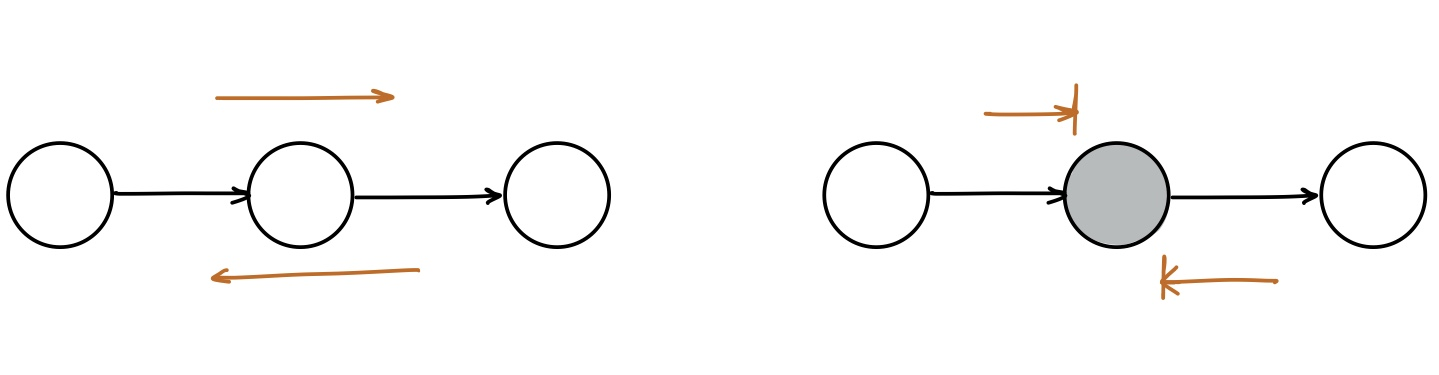
\includegraphics[scale=0.25]{img/bayes_ball_chain}
\end{center}
\paragraph{Common Cause}
\begin{center}
    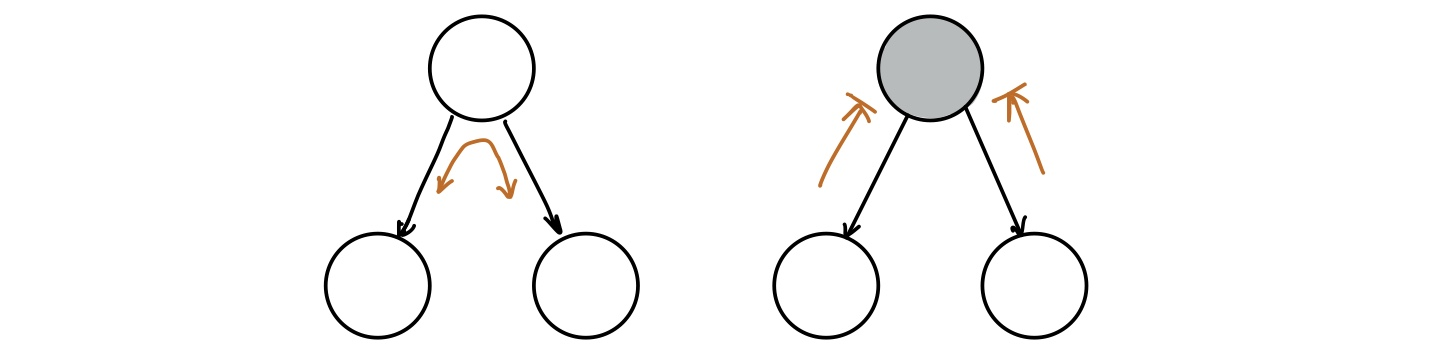
\includegraphics[scale=0.25]{img/bayes_ball_common_cause}
\end{center}
\paragraph{Explain Away}
\begin{center}
    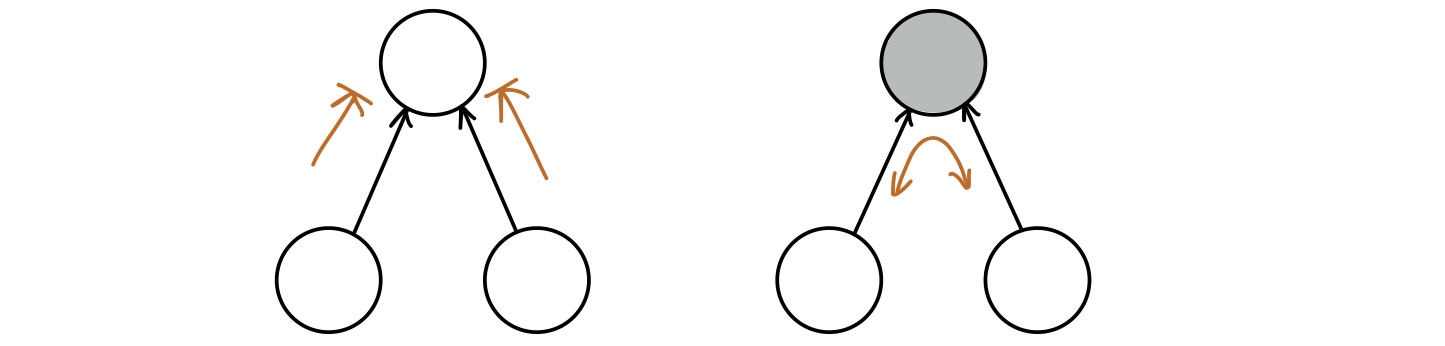
\includegraphics[scale=0.25]{img/bayes_ball_explain_away}
\end{center}
\paragraph{Linear}
\begin{center}
    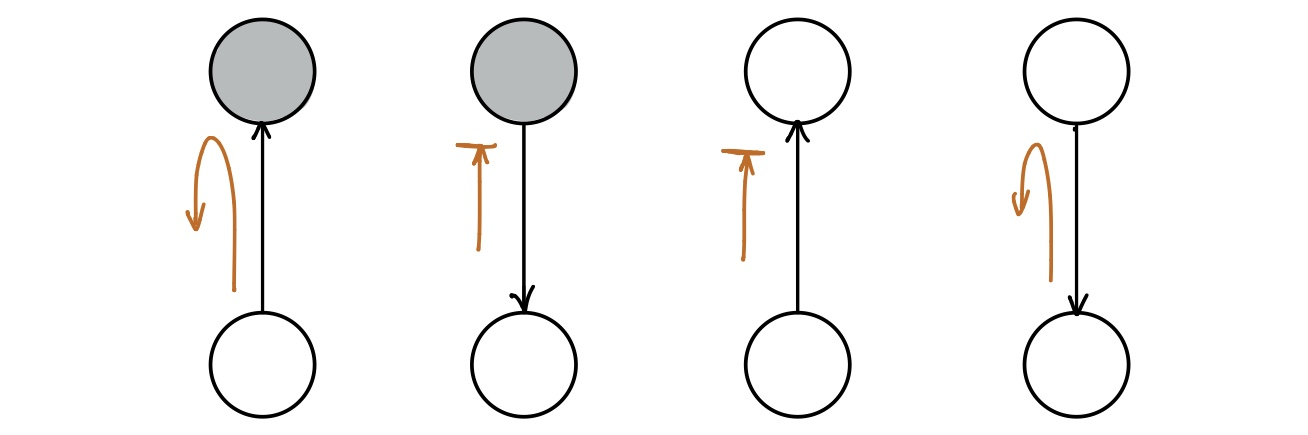
\includegraphics[scale=0.25]{img/bayes_ball_linear}
\end{center}

\subsection{Unobserved Variables}
Certain variables in our models may be unobserved , either some of the time or always, at training time or at test time. Graphically, we use shading to indicate observation.
\subsubsection{Partially Unobserved Variables}\footnote{An concrete example would be hospital data, where typically a large proportion of the data is missing. }
If variables are occasionally unobserved hen they are missing data, e.g., undefined inputs, missing class labels, erroneous target values. In this case, we can still model the joint distribution, but we marginalize the missing values
\begin{align}
    \ell(\theta ; \mathcal{D})&=\sum_{\text {complete }} \log p\left(x^{c}, y^{c} | \theta\right)+\sum_{\text {missing }} \log p\left(x^{m} | \theta\right) \\
    &=\sum_{\text {complete }} \log p\left(x^{c}, y^{c} | \theta\right)+\sum_{\text {missing }} \log \sum_{y} p\left(x^{m}, y | \theta\right)
\end{align}

\subsubsection{Latent Variables}
Above we discussed the case where some data are non-deterministically unobserved. Latent variables refers to those that \textit{\textbf{never observed}}. The handling of the latent variables depends on where it appears in our model,
\begin{itemize}
    \item If we never condition on it when computing the probability of the variables we do observe, then we can just forget about it and integrate it out. For example, given $y$, $x$ we fit the model
        \begin{equation}
            p(z, y | x)=p(z | y) p(y | x, w) p(w)
        \end{equation}
    \item If $z$ is not a leaf node, marginalizing over it will induce dependencies between its children. For example, given $y, x$ we can fit the model 
        \begin{equation}
            p(y | x)=\sum_{z} p(y | x, z) p(z)
        \end{equation}
\end{itemize}

\subsubsection{Mixture Models}
In this case, we are looking at data that has no input on class information. We can sum the labels out,
\begin{equation}
    p(x | \theta)=\sum_{k=1}^{K} p\left(z=k | \theta_{z}\right) p\left(x | z=k, \theta_{k}\right)
\end{equation}
where bayes rule comes in handy for calculating the posterior (class responsibilities) of the mixture component given some data, i.e., 
\begin{equation}
    p\left(z=k | x, \theta_{z}\right)=\frac{p\left(z=k | \theta_{z}\right) p_{k}\left(x | \theta_{k}\right)}{\sum_{j} p\left(z=j | \theta_{z}\right) p_{j}\left(x | \theta_{j}\right)}
\end{equation} 
%
%\paragraph{(Example) K-Gaussian Mixture Model}
%\begin{itemize}
%    \item The density model $p(x|\theta)$ is the marginal density. 
%\end{itemize}

\subsection{Examples}
\subsubsection{Second-order Markov Chain}
Consider the model
\begin{equation}
    p\left(\mathbf{x}_{1: T}\right)=p\left(x_{1}, x_{2}\right) p\left(x_{3} | x_{1}, x_{2}\right) p\left(x_{4} | x_{2}, x_{3}\right) \dots = p\left(x_{1}, x_{2}\right) \prod_{t=3}^{T} p\left(x_{t} | x_{t-1}, x_{t-2}\right)
\end{equation}
which has the graphical representation (double circles mean ``observed'' here)
\begin{center}
    \begin{tikzpicture}[scale=0.2]
    \tikzstyle{every node}+=[inner sep=0pt]
    \draw [black] (14.9,-18.4) circle (3);
    \draw (14.9,-18.4) node {$x_1$};
    \draw [black] (14.9,-18.4) circle (2.4);
    \draw [black] (23.7,-25.3) circle (3);
    \draw (23.7,-25.3) node {$x_2$};
    \draw [black] (23.7,-25.3) circle (2.4);
    \draw [black] (32.1,-18.4) circle (3);
    \draw (32.1,-18.4) node {$x_3$};
    \draw [black] (32.1,-18.4) circle (2.4);
    \draw [black] (41.2,-25.3) circle (3);
    \draw (41.2,-25.3) node {$x_4$};
    \draw [black] (41.2,-25.3) circle (2.4);
%    \draw [black] (49.2,-18.4) circle (3);
    \draw (49.2,-18.4) node {$...$};
    \draw [black] (17.26,-20.25) -- (21.34,-23.45);
    \fill [black] (21.34,-23.45) -- (21.02,-22.56) -- (20.4,-23.35);
    \draw [black] (26.02,-23.4) -- (29.78,-20.3);
    \fill [black] (29.78,-20.3) -- (28.85,-20.43) -- (29.48,-21.2);
    \draw [black] (34.49,-20.21) -- (38.81,-23.49);
    \fill [black] (38.81,-23.49) -- (38.47,-22.61) -- (37.87,-23.4);
    \draw [black] (43.47,-23.34) -- (46.93,-20.36);
    \fill [black] (46.93,-20.36) -- (46,-20.5) -- (46.65,-21.26);
    \draw [black] (17.9,-18.4) -- (29.1,-18.4);
    \fill [black] (29.1,-18.4) -- (28.3,-17.9) -- (28.3,-18.9);
    \draw [black] (26.7,-25.3) -- (38.2,-25.3);
    \fill [black] (38.2,-25.3) -- (37.4,-24.8) -- (37.4,-25.8);
    \end{tikzpicture}
\end{center}
we notice that this model essentially assumes ``the present depends on the past only through the current state as well as the last one.''

\subsubsection{Hidden Markov Models (HMMs)}
HMM is a statistical model in which a system being modelled is assumed to be a Markov Process\footnote{In continuous time, the Markov Chain model is known as Markov Process} with un-observed states. Here is the graphical model, where double circles mean ``observed'' here:
\begin{center}
    \begin{tikzpicture}[scale=0.2]
        \tikzstyle{every node}+=[inner sep=0pt]
        \draw [black] (13.9,-20.9) circle (3);
        \draw (13.9,-20.9) node {$z_1$};
        \draw [black] (24.7,-20.9) circle (3);
        \draw (24.7,-20.9) node {$z_2$};
        \draw [black] (35,-20.9) circle (3);
        \draw (35,-20.9) node {$z_3$};
        \draw [black] (45.7,-20.9) circle (3);
        \draw (45.7,-20.9) node {$z_4$};
        \draw [black] (56.5,-20.9) circle (3);
        \draw (56.5,-20.9) node {$z_5$};
%        \draw [black] (67,-20.9) circle (3);
        \draw (67,-20.9) node {$...$};
        \draw [black] (13.9,-31.5) circle (3);
        \draw (13.9,-31.5) node {$x_1$};
        \draw [black] (13.9,-31.5) circle (2.4);
        \draw [black] (24.7,-31.5) circle (3);
        \draw (24.7,-31.5) node {$x_2$};
        \draw [black] (24.7,-31.5) circle (2.4);
        \draw [black] (35,-31.5) circle (3);
        \draw (35,-31.5) node {$x_3$};
        \draw [black] (35,-31.5) circle (2.4);
        \draw [black] (45.7,-31.5) circle (3);
        \draw (45.7,-31.5) node {$x_4$};
        \draw [black] (45.7,-31.5) circle (2.4);
        \draw [black] (56.5,-31.5) circle (3);
        \draw (56.5,-31.5) node {$x_5$};
        \draw [black] (56.5,-31.5) circle (2.4);
        \draw [black] (16.9,-20.9) -- (21.7,-20.9);
        \fill [black] (21.7,-20.9) -- (20.9,-20.4) -- (20.9,-21.4);
        \draw [black] (27.7,-20.9) -- (32,-20.9);
        \fill [black] (32,-20.9) -- (31.2,-20.4) -- (31.2,-21.4);
        \draw [black] (38,-20.9) -- (42.7,-20.9);
        \fill [black] (42.7,-20.9) -- (41.9,-20.4) -- (41.9,-21.4);
        \draw [black] (48.7,-20.9) -- (53.5,-20.9);
        \fill [black] (53.5,-20.9) -- (52.7,-20.4) -- (52.7,-21.4);
        \draw [black] (59.5,-20.9) -- (64,-20.9);
        \fill [black] (64,-20.9) -- (63.2,-20.4) -- (63.2,-21.4);
        \draw [black] (13.9,-23.9) -- (13.9,-28.5);
        \fill [black] (13.9,-28.5) -- (14.4,-27.7) -- (13.4,-27.7);
        \draw [black] (24.7,-23.9) -- (24.7,-28.5);
        \fill [black] (24.7,-28.5) -- (25.2,-27.7) -- (24.2,-27.7);
        \draw [black] (35,-23.9) -- (35,-28.5);
        \fill [black] (35,-28.5) -- (35.5,-27.7) -- (34.5,-27.7);
        \draw [black] (45.7,-23.9) -- (45.7,-28.5);
        \fill [black] (45.7,-28.5) -- (46.2,-27.7) -- (45.2,-27.7);
        \draw [black] (56.5,-23.9) -- (56.5,-28.5);
        \fill [black] (56.5,-28.5) -- (57,-27.7) -- (56,-27.7);
    \end{tikzpicture}
\end{center}
where
\begin{itemize}
    \item $z_t$ are hidden states taking on one of $K$ discrete values
    \item $x_t$ are observed variables taking on values in any space.
\end{itemize}
The above graph factorizes into
\begin{equation}
    p\left(X_{1: T}, Z_{1: T}\right)=p\left(Z_{1: T}\right) p\left(X_{1: T} | Z_{1: T}\right)=p\left(Z_{1}\right) \prod_{t=2}^{T} p\left(Z_{t} | Z_{t-1}\right) \prod_{t=1}^{T} p\left(X_{t} | Z_{t}\right)
\end{equation}

\section{Lecture 4 - Exact Inference}
\subsection{Variable Elimination}
\subsubsection{(Simple Example) Chain}
The example that we will consider is the simple chain
\begin{equation}
    A \rightarrow B \rightarrow C \rightarrow D
\end{equation}
where we want to compute $P(D)$, with no observation\note{No observations for other variables means that we have no `evidence' for other variables. } for other variables. We have\note{$X_F$  is the set of variable that we are interested in, $X_E$ is evidence, and $X_R$ is the set of extraneous variables, i.e. what we marginalize out}
\begin{equation}
    X_{F}=\{D\}, X_{E}=\{\}, X_{R}=\{A, B, C\}
\end{equation}
The graphical model gives the factorization of
\begin{equation}
    p(A, B, C, D)=p(A) p(B | A) p(C | B) p(D | C)
\end{equation}
thus, if we want to find $p(D)$ we can marginalize over all other variables, i.e.
\begin{align}
    p(D)&=\sum_{A, B, C} p(A, B, C, D) \\
    &=\sum_{C} \sum_{B} \sum_{A} p(A) p(B | A) p(C | B) p(D | C)
\end{align}
If we marginalize the above the na\"ive way, then it cost exponentially $\mathcal{O}(k^n)$. Thus, we need to find a \textit{\textbf{elimination ordering}} that gives us a smaller runtime complexity. We can reduce the complexity by first computing terms that appear across the other marginalization sums, \note{Here $\phi$ means factor, an non-normalized ``pmf''}
\begin{align}
    \phi(D) 
    &= \sum_C p(D|C) \sum_B p(C|B) \sum_A p(A)p(B|A) \\
    &= \sum_C p(D|C) \sum_B p(C|B) \phi(B) \\
    &= \sum_C p(D|C) \phi(C)
\end{align}

\subsection{Sum-Product Inference}
Let $X = Z \cup Y \wedge Z \cap Y = \emptyset$ be a set of random variables. \note{Here $Y$ is the set that we want to do inference on and thus we are marginalizing over everything in $Z$}. Then, to compute $P(Y)$ for a directed and undirected \unsure{how to generalize to undirected graph?} model could be achieved by the sum product inference algorithm
\begin{equation}
    \tau(Y)=\sum_{z}\prod_{\phi \in \Phi} \phi\left(\mathrm{Scope}(\phi) \cap Z, \mathrm{Scope}(\phi) \cap Y\right)\quad \forall Y
\end{equation}
where the scope for each $\phi$ simply means the set of all random variables that have appeared in that specific $\phi$, and $\Phi$ denotes the set of all $\phi$'s.

\subsubsection{SP - Inference in  Directed Models}
In a directed model, the $\Phi$ is given by the conditional probability distributions for all variables, i.e.
\begin{equation}
    \Phi=\left\{\phi_{x_{i}}\right\}_{i=1}^{N}=\left\{p\left(x_{i} | \text { parents }\left(x_{i}\right)\right)\right\}_{i=1}^{N}
\end{equation}
The resulting term $\tau(Y)$ will be automatically normalized.

\subsubsection{SP - Inference in Undirected Models}
For undirected models, $\Phi$ is given by the set of un-normalized potentials, and we \textit{\textbf{must}} normalize the resulting $\tau(Y)$ by $\sum_Y \tau(y)$

\subsubsection{(Example) Directed Graph}
We have the following factorization of the joint distribution
\begin{equation}
    p(C, D, I, G, S, L, H, J)=p(C) p(D | C) p(I) p(G | D, I) p(L | G) P(S | I) p(J | S, L) p(H | J, G)
\end{equation}
and we will need the following potentials
\begin{equation}
    \Phi =\{\phi(C), \phi(C, D), \phi(I), \phi(G, D, I), \phi(L, G), \phi(S, I), \phi(J, S, L), \phi(H, J, G)\}
\end{equation}
consider the problem where we want to infer $P(J)$ with elimination ordering $\prec_{\{C, D, I, H, G, S, L\}}$.\footnote{Note that what comes first in the ordering is the what we want to sum over in the inner most summation} Then,
\begin{align}
    p(J) &= \sum_{L} \sum_{S} \phi(J, L, S) \sum_{G} \phi(L, G) \sum_{H} \phi(H, G, J) \sum_{I} \phi(S, I) \phi(I) \sum_{D} \phi(G, D, I) \sum_{C} \phi(C) \phi(C, D)\\
    &= ... \underbrace{\sum_{C} \phi(C) \phi(C, D)}_{\tau(D)} \\
    &= ... \underbrace{\sum_{D} \phi(G, D, I) \tau(D)}_{\tau(G, I)} \\
    &= ... \underbrace{\sum_{I} \phi(S, I) \phi(I) \tau(G, I)}_{\tau(S, G)} \\
    &= ... \underbrace{\tau(S, G)\sum_{H} \phi(H, G, J)}_{\tau(S, G)\tau(G, J)} ~~~~ \text{// Note that $\tau(S,G)$ doesn't contain $H$}\\
    &= ... \underbrace{\sum_{G} \phi(L, G) \tau(S, G) \tau(G, J)}_{\tau(J, L, S)} \\
    &= ... \underbrace{\sum_{S} \phi(J, L, S) \tau(J, L, S)}_{\tau(J, L)} \\
    &= ... \underbrace{\sum_{L} \tau(J, L)}_{\tau(J)}\\
    &= \tau(J)
\end{align}

\subsubsection{Complexity of VE}
The complexity of VE is 
\begin{equation}
    \mathcal{O}\left(m k^{N_{\max }}\right)
\end{equation}
where
\begin{itemize}
    \item $m = |\Phi|$ is the number of initial factors, i.e. the number of terms in the original factorization of the joint probability (given the graphical model)
    \item $k$ is the number of states each random variable takes (assumed to be equal here)
    \item $N_i$ is the number of random variables inside each sum $\sum_i$ \textit{at the time of marginalization}
    \item $N_{max} \triangleq \max_i N_i$ is the number of random variables inside the largest sum. (Inner sums are counted as one term all together)
\end{itemize}


\section{Lecture 5 - Message passing, Hidden Markov Models, and Sampling}
\subsection{Message Passing}
\subsubsection{Belief Propagation: Motivation and Definitions}
Our goal is to compute the marginal of every variable in graph $p(x_i), \forall x_i \in X$. Notice that in a tree, we have\info{Below, $T$ means the set of edges in the tree}
\begin{equation}
    P\left(X_{1: n}\right)=\frac{1}{Z} \prod_{k \in\{1,\dots,n\}} \phi\left(x_{k}\right) \prod_{(i, j) \in T} \phi_{i, j}\left(x_{i}, x_{j}\right)
\end{equation}
and thus, if we want to compute $P(X_1)$ we can marginalize out all other variables
\begin{align}
    P(X_1) = \sum_{x_2,\dots,x_n} P(X_{1:n}) 
    &= \sum_{x_2,\dots,x_n} \frac{1}{Z} \prod_k \phi\left(x_{k}\right) \prod_{(i, j) \in T} \phi_{i, j}\left(x_{i}, x_{j}\right) \\
    &\propto \sum_{x_2,\dots,x_n}  \prod_k \phi\left(x_{k}\right) \prod_{(i, j) \in T} \phi_{i, j}\left(x_{i}, x_{j}\right)
\end{align}
Now that we have the goal, we can group what we want to compute into a more structured representation, where we define \textit{\textbf{message-passing}} from variable $j$ to $i \in N(j)$ as
\begin{equation}
    m_{j \rightarrow i}\left(x_{i}\right)=\sum_{x_{j}} \phi_{j}\left(x_{j}\right) \phi_{i j}\left(x_{i}, x_{j}\right) \prod_{k \in N(j) \neq i} m_{k \rightarrow j}\left(x_{j}\right)
\end{equation}

\subsubsection{Belief Propagation Algorithm}
%\unsure{What is meant here in steps 2 and 3?}
\begin{enumerate}
    \item Choose an root $r$ arbitrarily, 
    \item Pass messages from leaves to $r$
    \item Pass messages from $r$ to leaves\info{Step 2 and 3 here so that we will compute all the $m_{i \rightarrow j}$, $\forall (i, j)$, $(j, i)\in T$, after which we can use them to calculate the marginals using formula in step 4}
    \item Compute
        \begin{equation}
            p\left(x_{i}\right) \propto \phi_{i}\left(x_{i}\right) \prod_{j \in \mathcal{N}(i)} m_{j \rightarrow i}\left(x_{i}\right), \forall_{i}
        \end{equation}
        \info{Notice that the idea is that we want to calculate \textit{\textbf{all}} of the marginals}
\end{enumerate}


\subsection{Inference in Hidden Markov Models}
There are the following four kinds of inference that we can do on a HMM, namely
\begin{itemize}
    \item \textit{\textbf{Filtering:}} Compute the belief state $p\left(z_{t} | \mathbf{x}_{1: t}\right)$ online. Notice that we call this inference operation filtering because this produces a result smoother than simply computing $p(z_t|\bx_{t})$.
    \item \textit{\textbf{Smoothing:}} Compute $p\left(z_{t} | \mathbf{x}_{1: T}\right)$ offline. Notice that this computation happens after all $\bx_{1:T}$ observations have been collected and hence is offline.\footnote{A very good intuitive example from KPM is that we have a detective investigating a crime scene, and as we gather more observation, the prediction that we make tends to be more and more certain and less `stochastic'.}\note{Definition in KPM is different from course note}
    \item \textit{\textbf{Fixed lag smoothing:}} Compute $p\left(z_{t-\ell} | \mathbf{x}_{1: t}\right)$, where $\ell>0$ is called the lag. Essentially, we want to do inference on the hidden state $z_\alpha$ and we wait until we observe all of $\bx_{1:\alpha + \ell}$ before we carry out the computation. 
    \item \textit{\textbf{Prediction:}} In this case, we want to compute $p\left(z_{t+h} | \mathbf{x}_{1: t}\right)$ for some $h > 0$. ($h$ is called the prediction horizon) Let's first take a look at the example where $h = 2$, then
    \begin{align}
        p(z_{t+2}|\bx_{1:t}) 
        &= \sum_{z_{t+1}}\sum_{z_t}p(z_t, z_{t+1}, z_{t+2}|\bx_{1:t}) \\
        &= \sum_{z_{t+1}}\sum_{z_t}p(z_t |\bx_{1:t})p(z_{t+1}|z_t, \bx_{1:t})p(z_{t+2}|z_{t+1}, z_{t}, \bx_{1:t}) \\
        &= \sum_{z_{t+1}} \sum_{z_{t}} p\left(z_{t+2} | z_{t+1}\right) p\left(z_{t+1} | z_{t}\right) p\left(z_{t} | \mathbf{x}_{1: t}\right)
    \end{align}
    where the last step of simplification could be easily justified using Bayes Ball rules. Above, we computed the prediction about the future hidden states, and it can be converted into prediction about the future observations using
    \begin{equation}
        p\left(\mathbf{x}_{t+h} | \mathbf{x}_{1: t}\right)=\sum_{z_{t+h}} p\left(\mathbf{x}_{t+h} | z_{t+h}\right) p\left(z_{t+h} | \mathbf{x}_{1: t}\right)
    \end{equation}
    which is called \textit{\textbf{Posterior Predictive Density}}.
\end{itemize}

\subsection{The Forward - Backward Algorithm}
Suppose that we want to find $p(z_t | x_{1:T}), \forall t$, then it can be broken down into two pieces
\begin{itemize}
    \item \textit{\textbf{Forward Filtering:}} Compute $p\left(z_{t}, x_{1: t}\right) \quad \forall t$, which effectively is the probability of the hidden state $z_t$ given all past observations, up to including $x_t$. 
    \item \textbf{\textit{Backward Filtering:}} Compute $p\left(x_{1+t: T} | z_{t}\right)\quad \forall t$, which computes the probability of \textit{all} future observations from $x_{t+1}$ up to including $x_T$ given the current hidden state, i.e. $z_t$.
\end{itemize}
Then, the complete smoothing $p(z_t | x_{1:T})$\note{This is called \textbf{Latent sequence given observations in HMM} in the course notes} could be computed as
\begin{align}
    p\left(z_{t} | x_{1: T}\right)
    &= p\left(x_{1:T}\right)p\left(z_{t}, x_{1: T}\right) \\
    &\propto p\left(z_{t}, x_{1: T}\right) \\
    &=p\left(z_{t}, x_{1: t}\right) p\left(x_{t+1: T} | z_{t}, x_{1: t}\right) \\
    &=p\left(z_{t}, x_{1: t}\right) p\left(x_{t+1: T} | z_{t}\right) && \text{// By Bayes Ball} \\
    &=(\text{Forward Recursion})(\text{Backward Recursion})
\end{align}

\subsubsection{Forward Filtering Recursion}
%There are two steps that we will do in this recursion, called predict-update cycle\info{From KPM}
%\begin{itemize}
%    \item \textit{\textbf{One step ahead predictive density}} can be computed as
%    \begin{align}
%        p\left(z_{t}=j | \mathbf{x}_{1: t-1}\right)
%        &= \sum_i p(z_t = j, z_{t - 1} = i | \bx_{1:t - 1}) \\
%        &= \sum_i p(z_t = j| z_{t - 1}= i, \bx_{1:t - 1})p(z_{t - 1} = i| \bx_{1:t - 1}) \\
%        &= \sum_{i} p\left(z_{t}=j | z_{t-1}=i\right) p\left(z_{t-1}=i | \mathbf{x}_{1: t-1}\right)
%    \end{align}
%    \item \textit{\textbf{Update Step}} is where we absorb the observed data form time $t$ using the Bayes Rule
%    \begin{align}
%        \alpha_{t}(j) 
%        &\triangleq p\left(z_{t}=j | \mathbf{x}_{1: t}\right)=p\left(z_{t}=j | \mathbf{x}_{t}, \mathbf{x}_{1: t-1}\right) \\
%        &= \frac{1}{Z_{t}} p\left(\mathbf{x}_{t} | z_{t}=j, \cancel{\mathbf{x}_{1: t-1}}\right) p\left(z_{t}=j | \mathbf{x}_{1: t-1}\right)
%    \end{align}
%    where
%    \begin{equation}
%        Z_{t} \triangleq p\left(\mathbf{x}_{t} | \mathbf{x}_{1: t-1}\right)=\sum_{j} p\left(z_{t}=j | \mathbf{x}_{1: t-1}\right) p\left(\mathbf{x}_{t} | z_{t}=j\right)
%    \end{equation}
%\end{itemize}
%Below is the version from course notes.\unsure{What is the connection?}
\begin{align}
    \alpha_t(z_t) = p\left(z_{t}, x_{1: t}\right)
    &=\sum_{z_{t-1}} p\left(z_{t-1}, z_{t}, x_{1: t}\right) \\
    &= \sum_{z_{t-1}} p\left(x_{t} | z_{t-1}, z_{t}, x_{1: t-1}\right) p\left(z_{t} | z_{t-1}, x_{1: t-1}\right) \underbrace{p\left(z_{t-1}, x_{1: t-1}\right)}_{ = \alpha_{t - 1}(z_{t - 1})}\\
    \implies &\alpha_{t}\left(z_{t}\right)=p\left(x_{t} | z_{t}\right) \sum_{z_{t-1}} p\left(z_{t} | z_{t-1}\right) \alpha_{t-1}\left(z_{t-1}\right)
\end{align}
Notice that our forward recursion contains our emission, $p(x_t | z_t)$ and transition $p(z_t | z_{t - 1})$. The base case of the recursion could be unwinded into
\begin{equation}
    \alpha_{1}\left(z_{1}\right)=p\left(z_{1}, x_{1}\right)=p\left(z_{1}\right) p\left(x_{1} | z_{1}\right)
\end{equation}


\subsubsection{Backward Filtering Recursion}
\begin{align}
    p\left(x_{t+1: T} | z_{t}\right)
    &=\sum_{z_{t+1}} p\left(z_{t+1}, x_{t+1: T} | z_{t}\right) \\
    &= \sum_{z_{t+1}} p\left(x_{t+2: T} | z_{t+1}, z_{t}, x_{t+1}\right) p\left(x_{t+1} | z_{t+1}, z_{t}\right) p\left(z_{t+1} | z_{t}\right) \\
    \implies &\beta_{t}\left(z_{t}\right)=\sum_{z_{t+1}} \underbrace{ p\left(x_{t+2 : T} | z_{t+1}\right)}_{ = \beta_{t +1}(z_{t + 1})} p\left(x_{t+1} | z_{t+1}\right) p\left(z_{t+1} | z_{t}\right)
\end{align}
and hence if we recurse the above relationship, we will unwind to the base case
\begin{equation}
    \beta_{1}\left(z_{1}\right)=p\left(x_{3: T} | z_{2}\right) p\left(x_{2} | z_{2}\right) p\left(z_{2} | z_{1}\right)
\end{equation}


\subsection{Sampling}
\note{The word sample here refers to a single realization from a distribution rather than a set. }
The goal is to, 
\begin{itemize}
    \item Generate sample $\left\{x^{(r)}\right\}_{r=1}^{R}$ from a probability distribution $p(x)$, and/or
    \item Estimate expectations of functions $f(x)$ under some distribution $p(x)$, usually we want to estimate moments for a distribution
    \begin{equation}
        E=\underset{x \sim p(x)}{\mathbb{E}}[f(x)]=\int f(x) p(x) d x
    \end{equation}
\end{itemize}

\subsubsection{Ancestral Sampling}
\paragraph{Generating marginal samples} If you are only interested in sampling a particular set of nodes, you can simply sample from all the nodes jointly, then ignore the nodes you don't need.

\paragraph{Generating conditional samples} If you want to sample conditional on a node with no parents, that's also easy - you can simple do ancestral sampling starting from the nodes you have. \newline \newline
\textit{\textbf{(\#! Important:)}} However, to sample from a DAG conditional on leaf nodes is hard in the same way that inference is hard in general. E.g. sampling the unknown key in a crypto-system given the cypher-text but not knowing the plaintext. Finding ways to do this approximately is what a lot of the rest of the course will be about.

\subsubsection{Simple Monte Carlo}
\paragraph{(Definition) - Simple MC} Given $\left\{x^{(r)}\right\}_{r=1}^{R} \sim p(x)$, we want to estimate the expectation $\underset{x \sim p(x)}{\mathbb{E}}[f(x)]$.
\begin{equation}
    E=\underset{x \sim p(x)}{\mathbb{E}}[f(x)] \approx \frac{1}{R} \sum_{r=1}^{R} f\left(x^{(r)}\right)=\hat{E}
\end{equation}
\paragraph{Unbiasedness of MC}
\begin{align}
    \mathbb{E}_{x \sim p\left(\left\{x^{(i)}\right\}_{r=1}^{R}\right)}[\hat{E}]
    &=\mathbb{E}\left[\frac{1}{R} \sum_{r=1}^{R} f\left(x^{(r)}\right)\right] \\
    &= \frac{1}{R} \sum_{r=1}^{R} \mathbb{E}\left[f\left(x^{(r)}\right)\right]\\
    &= \frac{1}{R} \sum_{r=1}^{R} \underset{x \sim p(x)}{\mathbb{E}}[f(x)] \\
    &= \frac{R}{R} \underset{x \sim p(x)}{\mathbb{E}}[f(x)] \\
    &= E
\end{align}
\qed

\paragraph{Variance of MC}
\begin{align}
    \operatorname{var}[\hat{E}]
    &=\operatorname{var}\left[\frac{1}{R} \sum_{r=1}^{R} f\left(x^{(r)}\right)\right] \\
    &= \frac{1}{R^{2}} \operatorname{var}\left[\sum_{r=1}^{R} f\left(x^{(r)}\right)\right] \\
    &= \frac{1}{R^{2}} \sum_{r=1}^{R} \operatorname{var}\left[f\left(x^{(r)}\right)\right]\\
    &= \frac{1}{R}\operatorname{var}\left[f(x) \right]
\end{align}
We notice that the accuracy of MC estimates only depends on the variance of $f$, not on the dimension of $x$. Also, we the number of samples, $R$, increases, the variance $\hat{E}$ will decrease at a rate proportional to $\frac{1}{R}$.
\qed


\section{Lecture 7 - Stochastic Variational Inference (SVI/ADVI)}
\subsection{Motivation - Approximating Posterior Inference}
Notice that if we want to calculate the \textit{exact} posterior distribution, for example, 
\begin{equation}
    p(z | x)=\frac{p(x | z)}{p(x)}=\frac{p(x, z) p(z)}{\int p(x, z) dz}
\end{equation} 
the bottom integral over all possible states soon becomes intractable, making the computation of the entire posterior distribution intractable. Hence, instead, we will approximate the posterior inference with \textit{\textbf{variational methods}}. Generally speaking, it works as follows
\begin{enumerate}
    \item We introduce a family of distributions, with variational parameters $\phi$, denoted as $q_\phi$. 
    \item We want to encode a ``distance metric'' between $p(z|x)$ and $q_\phi(z)$.
    \item Try to minimize the proposed ``distance metric''.
\end{enumerate}
There are a few things to note
\begin{itemize}
    \item First, as we will soon see, we use a measure of closeness that is \textit{\textbf{not}} a distance metric. Also, using na\"ive distance metric could fail spectacularly (arbitrarily bad examples can be found if we use MSE).
    \item This formulation turns the Bayesian Inference into an optimization problem. If enough parts of the model is differentiable and could be well-approximated with Monte  Carlo, then we can use gradient based optimization methods to solve this problem scalably. 
\end{itemize}


\subsection{The Kullback-Leibler Divergence}
Suppose $q_\phi$ denotes a family of distributions with its own \textbf{variational parameters} $\phi$, and $p$ is some distribution. Then, the Kullback-Leibler divergence is defined as
\begin{align}
    D_{\mathrm{K L}}\left(q_{\phi}(z | x) \| p(z | x)\right)
    &=\int q_{\phi}(z | x) \log \frac{q_{\phi}(z | x)}{p(z | x)} d z \\
    &=\underset{z \sim q_{\phi}}{\mathbb{E}} \left[ \log \frac{q_{\phi}(z | x)}{p(z | x)} \right]
\end{align}

\paragraph{Properties} of KL Divergence
\begin{enumerate}
    \item $D_\kl (q_\phi || p) \geq 0$, non-negativeness
    \item $D_\kl (q_\phi || p) = 0 \iff q_\phi = p$
    \item $D_\kl (q_\phi || p) \neq D_\kl (p || q_\phi)$, i.e. KL Divergence is \textit{\textbf{not}} a metric distance. 
\end{enumerate}

\subsubsection{Expectation Propagation}
If we try to reverse the arguments, it leads to a different kind of variational inference that is called ``expectation propagation''. Typically, this leads to an algorithm that is more computationally expensive. 

\subsection{The Evidence Lower BOund (ELBO)}
\subsubsection{Definition and Equivalence Property}
We cannot minimize the KL divergence exactly\info{$D_\kl (q_\phi || p)$ is intractable because it contains $p(z|x)$, which is intractable.}, thus we introduce a function, ELBO, and try to minimize that. Notice that ELBO is equal to the actual KL divergence up to a constant. 
\begin{align}
    D_{\kl}\left(q_{\phi}(z | x) \| p(z | x)\right)
    &=\underset{z \sim q_{\phi}}{\mathbb{E}} \log \frac{q_{\phi}(z | x)}{p(z | x)} \\
    &= \underset{z \sim q_{\phi}}{\mathbb{E}}\left[\log \left(q_{\phi}(z | x) \cdot \frac{p(x)}{p(z, x)}\right)\right] \\
    &= \underset{z \sim q_{\phi}}{\mathbb{E}} \log \frac{q_{\phi}(z | x)}{p(z, x)}+\underset{z \sim q_{\phi}}{\mathbb{E}} \log p(x) \\
    &= -\mathcal{L}(\phi; x) + \log p(x)
\end{align}
where $\mathcal{L}(\phi; x) = -\underset{z \sim q_{\phi}}{\mathbb{E}} \log \frac{q_{\phi}(z | x)}{p(z, x)}$ is defined as the ELBO. If we re-arrange what we have above,
\begin{equation}
    \log p(x) = \mathcal{L}(\phi ; x)+D_{\kl}\left(q_{\phi}(z | x) \| p(z | x)\right)
\end{equation}
and we notice that $D_{\kl}\left(q_{\phi}(z | x) \| p(z | x)\right) \geq 0$, it then follows that 
\begin{equation}
    \mathcal{L}(\phi ; x) \leq \log p(x)
\end{equation}
Hence, to minimize the KL divergence we need to maximize the ELBO, and they are equivalent.

\subsubsection{Optimization goal of ELBO}
We have, by definition of ELBO, that
\begin{align}
    \mathcal{L}(\phi; x)
    &= -\underset{z \sim q_{\phi}}{\mathbb{E}} \log \frac{q_{\phi}(z | x)}{p(x, z)} \\
    &= \underset{z \sim q_{\phi}}{\mathbb{E}}\left[\log p(x, z)-\log q_{\phi}(z | x)\right]
\end{align}
Recall, that our goal is to use gradient based methods to optimize this objective, meaning that we have to somehow compute, estimate to be precise in this case, the gradient of ELBO $\mathcal{L}(\phi; x)$
\begin{equation}
    \nabla_{\phi} \mathcal{L}(\phi)=\nabla_{\phi} \mathbb{E}_{z \sim q_{\phi}(z | x)}\left[\log p(x, z)-\log q_{\phi}(z | x)\right]
\end{equation}
and we know from a previous lecture that one can get an unbiased estimator of any expectation as long as we can sample from the distribution and evaluate the function, using simple Monte Carlo.

\subsubsection{Pathwise Gradient}
Above, we saw that the objective is the gradient over an expectation and we now would like to make it an expectation over gradient. In general, such swapping is not allowed and we can only do so if the distribution we're taking the expectation over \textit{\textbf{does not}} depend on the parameter, i.e. $\phi$. Our goal is now to factor our the randomness of from $q$, and put it into a parameterless, fixed source of noice $p(\varepsilon)$. Formally, we need to find function $T(\phi,\varepsilon )$ such that 
\begin{equation}
    \begin{rcases}
        \varepsilon \sim p(\varepsilon ) \\
        z = T(\phi,\varepsilon ) 
    \end{rcases}
    \implies z\sim q_\phi(z)
\end{equation}
We usually start with $p(\varepsilon )$ being uniform or normal. Indeed it is not always easy to find these functions\footnote{\url{http://blog.shakirm.com/2015/10/machine-learning-trick-of-the-day-4-reparameterisation-tricks/}} and as a easy concrete example, we know
\begin{equation}
    \begin{rcases}
        \varepsilon \sim \mathcal{N}(\varepsilon | 0, 1) \\
        z = \sigma \varepsilon + \mu
    \end{rcases}
    \implies z\sim \mathcal{N}(z | \mu, \sigma )
\end{equation}
Then, by applying the trick we know,
\begin{align}
    \nabla_{\phi} \mathcal{L}(\phi)
    &=\nabla_{\phi} \mathbb{E}_{z \sim q_{\phi}(z | x)}\left[\log p(x, z)-\log q_{\phi}(z | x)\right] \\
    &=\nabla_{\phi} \mathbb{E}_{\varepsilon \sim p(\varepsilon)}\left[\log p(x, T(\phi, \varepsilon))-\log q_{\phi}(T(\phi, \varepsilon) | x)\right] \\
    &=\mathbb{E}_{\varepsilon \sim p(\varepsilon)} \nabla_{\phi}\left[\log p(x, T(\phi, \varepsilon))-\log q_{\phi}(T(\phi, \varepsilon) | x)\right]
\end{align}

\subsection{Tutorial}
\subsubsection{Derivation Using Jensen's Inequality}
Recall that by when Jensen's inequality is applied to probability distributions, we know that when $f$ is concave,
\begin{equation}
    f(\mathbb{E}[X]) \geq \mathbb{E}[f(X)]
\end{equation}
Then, for the log probability of the observations,
\begin{align}
    \log p(x) 
    &= \log \int p(x,z) dz \\
    &= \log \int p(x,z) \frac{q_\phi(z|x)}{q_\phi(z|x)} dz \\
    &= \log \mathbb{E}_{z\sim q_\phi} \frac{p(x,z)}{q_\phi(z|x)}
\end{align}
where we apply Jensen's Inequality
\begin{align}
    \implies \underset{z \sim q_{\phi}}{\mathbb{E}} \frac{p(x, z)}{q_{\phi}(z | x)} 
    &\geq \underset{z \sim q_{\phi}}{\mathbb{E}} \log \frac{p(x, z)}{q_{\phi}(z | x)} \\
    &= -\underset{z \sim q_{\phi}}{\mathbb{E}} \log \frac{q_{\phi}(z | x)}{p(x, z)} \\
    &=\mathcal{L}(\phi ; x)
\end{align}

\subsubsection{Interpretations of ELBO}
For the ELBO defined as
\begin{equation}
    \mathrm{ELBO} \triangleq \mathcal{L}(\phi ; x) =-\underset{z \sim q_{\theta}}{\mathbb{E}} \log \frac{q_{\phi}(z | x)}{p(x, z)}
\end{equation}
we have
\begin{enumerate}
    \item The most general interpretation is just breaking up the logarithm. We have
    \begin{align}
        \mathcal{L}(\phi ; x)
        &=-\underset{z \sim q_{\phi}}{\mathbb{E}} \log \frac{q_{\phi}(z | x)}{p(x, z)} \\
        &= \underset{z \sim q_{\phi}}{\mathbb{E}} \log \frac{p(x, z)}{q_{\phi}(z | x)} \\
        &= \underset{z \sim q_{\phi}}{\mathbb{E}} \log \frac{p(z) p(x | z)}{q_{\phi}(z | x)} \\
        &= \underset{z \sim q_{\phi}}{\mathbb{E}}\left[\log p(x | z)+\log p(z)-\log q_{\phi}(z | x)\right]
    \end{align}
    \item We can try to write this using entropy as 
    \begin{equation}
        \mathcal{L}(\phi ; x) = \underset{z \sim q_{\phi}}{\mathbb{E}}[\log p(x | z)+\log p(z)] \mathcal{H}\left(q_{\phi}(z | x)\right)
    \end{equation}
    \item We can frame ELBO as a trade off
    \begin{equation}
        \mathcal{L}(\phi ; x) = \underbrace{\underset{z \sim q_{\phi}}{\mathbb{E}}[\log p(x | z)]}_{(\dag)} - \underbrace{D_{K L}\left(q_{\phi}(z | x) \| p(z)\right)}_{(\ddag)}
    \end{equation}
    \begin{itemize}
        \item $(\dag)$ is ``reconstruction likelihood'', i.e. how probable is $x$ given $z$, which encourages the model to choose the distribution which best reconstructs the data. 
        \item $(\ddag)$ acts as regularization, enforcing the idea that our parametrization shouldn't move us too far from the true distribution. 
    \end{itemize}
\end{enumerate}


























\end{document}
